\documentclass[11pt]{amsart}
\usepackage[margin=1in]{geometry}


\usepackage{microtype}
\usepackage{amsmath,amssymb,amsthm}
\usepackage{graphicx}
\usepackage{xcolor}
\usepackage{booktabs}
\usepackage{array}
\usepackage[numbers,sort&compress]{natbib}
\usepackage[colorlinks=true,linkcolor=blue!50!black,citecolor=blue!50!black,urlcolor=blue!50!black]{hyperref}
\usepackage[capitalise,noabbrev]{cleveref}

% AUTO-GENERATED by experiments/run_all.py -- do not edit by hand
\newcommand{\benchCIHi}{0.807}
\newcommand{\benchCILo}{0.642}
\newcommand{\benchFamilies}{9}
\newcommand{\benchGM}{0.716}
\newcommand{\benchGMReduction}{28}
\newcommand{\benchLossFamilies}{F3 corners+arcs, F4 line+bumps, F7 Fourier star (closed), F9 mixed trajectory}
\newcommand{\benchLosses}{9}
\newcommand{\benchN}{1000}
\newcommand{\benchPairs}{45}
\newcommand{\benchWilcoxonP}{4.3\times10^{-4}}
\newcommand{\benchWilcoxonW}{215}
\newcommand{\benchWins}{36}
\newcommand{\clsEuclidMild}{87.3}
\newcommand{\clsEuclidStrong}{83.3}
\newcommand{\clsHybridMild}{100.0}
\newcommand{\clsHybridStrong}{89.3}
\newcommand{\clsN}{150}
\newcommand{\clsPerClass}{30}
\newcommand{\clsProcrustesMild}{100.0}
\newcommand{\clsProcrustesStrong}{98.0}
\newcommand{\clsPureMild}{100.0}
\newcommand{\clsPureStrong}{89.3}
\newcommand{\clsTurningMild}{100.0}
\newcommand{\clsTurningStrong}{99.3}
\newcommand{\convOrderMax}{1.01}
\newcommand{\convOrderMin}{1.00}
\newcommand{\cornerPinnedVsRDP}{+36}
\newcommand{\cornerUnpinnedVsRDP}{+3153}
\newcommand{\cqBeatsOpt}{4}
\newcommand{\cqOneGM}{2.007}
\newcommand{\cqUnpinnedGM}{0.833}
\newcommand{\dimpleHybrid}{0.0522}
\newcommand{\dimplePure}{0.351}
\newcommand{\dimpleReduction}{85}
\newcommand{\dimpleTurningBase}{0.0040}
\newcommand{\distEarlyLate}{0.283}
\newcommand{\distEarlyLateHybrid}{0.161}
\newcommand{\distUS}{3.1\times10^{-7}}
\newcommand{\gapDOne}{0.093}
\newcommand{\gapDSix}{0.263}
\newcommand{\gapRatio}{2.8}
\newcommand{\gompertzSlopeEndDeg}{0.019}
\newcommand{\invarianceResample}{0.0012}
\newcommand{\invarianceSimilarity}{2.5\times10^{-14}}
\newcommand{\medGompertz}{-0.0320}
\newcommand{\medXcube}{0.553815}
\newcommand{\medXsq}{0.390388}
\newcommand{\noiseCleanHybrid}{1.320}
\newcommand{\noiseCleanKmax}{0.340}
\newcommand{\noiseCleanMedian}{0.862}
\newcommand{\noiseKmaxRatioMax}{3.9}
\newcommand{\noiseKmaxRatioMin}{1.7}
\newcommand{\noiseRawWorst}{1.29}
\newcommand{\noiseResampleTrials}{20}
\newcommand{\noiseTrials}{200}
\newcommand{\optRatioGM}{1.32}
\newcommand{\optRatioMax}{4.17}
\newcommand{\optRatioMin}{0.92}
\newcommand{\quartileDSix}{6.14}
\newcommand{\rdpOptRatioGM}{1.85}
\newcommand{\snapGM}{0.859}
\newcommand{\spiralCQHalfFifty}{4.28}
\newcommand{\spiralCQHalfThirty}{11.76}
\newcommand{\spiralCQOneFifty}{10.50}
\newcommand{\spiralCQOneThirty}{29.02}
\newcommand{\spiralRDPFifty}{6.76}
\newcommand{\spiralRDPThirty}{20.80}
\newcommand{\spiralRedRDPFifty}{37}
\newcommand{\spiralRedRDPThirty}{43}
\newcommand{\spiralRedUniformCQOneFifty}{49}
\newcommand{\spiralRedUniformCQOneThirty}{44}
\newcommand{\spiralUniformFifty}{20.59}
\newcommand{\spiralUniformThirty}{51.80}
\newcommand{\truncArcMid}{-1.47}
\newcommand{\truncDomainMid}{-1.50}
\newcommand{\truncMedian}{-0.62}
\newcommand{\uniformGM}{5.38}
\newcommand{\vwGM}{1.52}
\newcommand{\wOneIdentityMaxDiff}{2.6\times10^{-6}}
\newcommand{\xsqArcMid}{1.333}


\newtheorem{theorem}{Theorem}
\newtheorem{proposition}[theorem]{Proposition}
\newtheorem{lemma}[theorem]{Lemma}
\newtheorem{corollary}[theorem]{Corollary}
\theoremstyle{definition}
\newtheorem{definition}[theorem]{Definition}
\theoremstyle{remark}
\newtheorem{remark}[theorem]{Remark}

\newcommand{\dd}{\,\mathrm{d}}
\newcommand{\R}{\mathbb{R}}
\newcommand{\Wone}{\mathcal{W}_1}
\newcommand{\repo}{\url{https://github.com/mike8685/curvature-quantiles}}

\title[Curvature quantiles]{Curvature Quantiles: Turning as a Distribution Along Planar Curves, with an Application to Fixed-Budget Polyline Simplification}

\author{Michael J. Wish}
\address{Independent researcher, Odenton, Maryland, USA}
\email{michaelj.wish@gmail.com}

\date{Preprint, October 19, 2026. Draft for comment.}

\keywords{total absolute curvature, quantiles, turning function, Wasserstein distance, polygonal approximation, curve simplification}
\subjclass[2020]{53A04, 65D18, 68U05, 49Q22}

\begin{document}

\begin{abstract}
For a regular planar curve the measure $|\kappa|\dd s$ equals the total variation $|\dd\theta|$ of the tangent angle. Normalizing it gives a probability distribution of turning along the curve, and this note studies that distribution with the ordinary tools of descriptive statistics. Its median, the \emph{curvature median}, has a closed form on convex graphs: the tangent angle there is the arithmetic mean of the boundary tangent angles. On a single sigmoidal transition with equal boundary slopes it is the inflection point, but with square-root sensitivity to slope mismatch at the boundaries. Quantile gaps detect when a single median falls between two separated bends. The $L^1$ distance between quantile profiles is the Wasserstein-1 distance between turning distributions, is invariant under similarities and reparameterization, and on convex arcs reduces to the classical turning-function distance of Arkin et al.\ with fixed start point and rotation. Most of these objects are elementary and several are close to existing work, in particular Tumpach's curvature-based canonical parameterizations, which we credit and build on. Our main empirical contribution is a reproducible fixed-budget simplification benchmark. Placing $K$ vertices at equal quantiles of $|\kappa|^{1/2}\dd s$, the classical asymptotically optimal density, gives \benchGMReduction\% lower worst-case error than Ramer--Douglas--Peucker on average over \benchPairs{} curve/budget pairs (geometric-mean error ratio \benchGM, 95\% bootstrap interval [\benchCILo, \benchCIHi]), and comes within a geometric-mean factor of \optRatioGM{} of the exact dynamic-programming optimum over vertex subsets, versus \rdpOptRatioGM{} for Ramer--Douglas--Peucker. The method is fragile under measurement noise, where a smoothed Ramer--Douglas--Peucker remains better in our tests. All numbers are regenerated by the accompanying open-source code.
\end{abstract}

\maketitle

% =====================================================================
\section{Introduction}

What is the ``middle'' of a curve? The midpoint of the domain depends on coordinates. The arc-length midpoint is intrinsic, but it weights a long straight approach exactly as much as a tight hairpin. If the interest is in \emph{where the curve turns}, a natural answer is the point that splits the total turning in half. This note follows that thought to its routine consequences: once turning is treated as a probability distribution along the curve, medians, quantiles, quantile gaps, and transport distances come for free, and each has a concrete geometric meaning.

None of the ingredients are new on their own. The total absolute curvature $\int|\kappa|\dd s$ is classical \cite{fenchel1929,milnor1950}. Parameterizing a curve proportionally to curvature, and blending arc length with curvature, was studied by Tumpach \cite{tumpach2023canonical} (see also \cite{ciuclea2025geometric}), whose construction coincides with the cumulative distribution used here. The turning-function representation of shapes goes back at least to Zahn and Roskies \cite{zahn1972fourier} and Arkin et al.\ \cite{arkin1991metric}. That optimal polygonal approximation with a fixed number of vertices places vertices with density proportional to $|\kappa|^{1/2}$ is a classical asymptotic result \cite{fejestoth1948,mcclure1975,glasauer1996}, closely related to de Boor's equidistribution principle for knots \cite{deboor1974}.

What this note adds is a consistent statistical reading of these objects and a careful, reproducible measurement of what they are good for. Specifically:
\begin{enumerate}
\item closed-form curvature medians and quantiles on convex graphs (\cref{thm:monotone}), the inflection-point property for single transitions together with its square-root sensitivity to boundary-slope mismatch (\cref{thm:sigmoid,rem:sqrt}), and the quantile-gap diagnostic for multiple bends (\cref{sec:multi});
\item the observation that the quantile-profile distance is the Wasserstein-1 distance between turning distributions and, on convex arcs, coincides with the normalized turning-function distance of \cite{arkin1991metric} (\cref{prop:w1,prop:arkin});
\item a benchmark of equal-quantile resampling against Ramer--Douglas--Peucker (RDP) \cite{ramer1972,douglas1973}, Visvalingam--Whyatt (VW) \cite{visvalingam1993}, and the exact optimum over vertex subsets \cite{imai1986,perez1994,chin1996}, including the cases where it loses (\cref{sec:resampling}).
\end{enumerate}
We also report negative results plainly: the profile distance is a weaker stroke classifier than the signed turning function under strong perturbation (\cref{sec:classify}), and quantile resampling degrades faster than RDP under measurement noise (\cref{sec:noise-resample}). Code, data, and scripts that regenerate every table and figure are available at \repo.

% =====================================================================
\section{Definitions}\label{sec:defs}

Let $\gamma:[0,L]\to\R^2$ be a curve of length $L>0$ parameterized by arc length, piecewise $C^2$, with curvature $\kappa(s)$ and tangent angle $\theta(s)$, so that $\theta'(s)=\kappa(s)$ on smooth pieces. Write $u=s/L\in[0,1]$ for normalized arc length.

\begin{definition}[Turning distribution]
The \emph{total turning} is $K(\gamma)=\int_0^L|\kappa(s)|\dd s$. When $K>0$ the \emph{turning distribution} $\nu_\gamma$ is the probability measure on $[0,1]$ with cumulative distribution function
\[
F_\gamma(u)=\frac{1}{K(\gamma)}\int_0^{uL}|\kappa(s)|\dd s .
\]
Its quantile function is $P_\gamma(q)=\inf\{u: F_\gamma(u)\ge q\}$, the \emph{curvature quantiles} are the points $\gamma(L\,P_\gamma(q))$, and the \emph{curvature median} is the quantile at $q=\tfrac12$.
\end{definition}

A corner of exterior angle $\alpha$ contributes an atom of mass $\alpha/K$ to $\nu_\gamma$, so the definition covers polygons without change. $F_\gamma$ is, up to normalization, the curvature-proportional parameterization of \cite{tumpach2023canonical}.

\begin{definition}[Weighted and hybrid measures]
For an exponent $p>0$ and weight $\beta\ge0$ let
\[
\dd\mu_{p,\beta}=\frac{\dd s}{L}+\beta\,L^{p-1}|\kappa(s)|^{p}\dd s ,
\]
normalized to a probability measure. The factor $L^{p-1}$ makes the measure dimensionless, hence invariant under scaling. For $p=1$, $\beta$ has units of inverse radians and the curvature share of the mass is $\beta K/(1+\beta K)$; as $K\to0$ the measure degrades continuously to uniform arc length, so it remains defined on straight lines where $\nu_\gamma$ is not. The case $p=1$ is, up to reparameterizing the weight, the arc-length/curvature blend of \cite{tumpach2023canonical}.
\end{definition}

\begin{definition}[Profile distance]
For two curves with turning distributions $\nu_1,\nu_2$ on $[0,1]$,
\[
D(\gamma_1,\gamma_2)=\int_0^1\bigl|P_{\gamma_1}(q)-P_{\gamma_2}(q)\bigr|\dd q .
\]
$D_\beta$ denotes the same quantity for the hybrid measures with $p=1$.
\end{definition}

\begin{definition}[Quantile gap]
For $0<h<\tfrac12$, $G_h(\gamma)=P_\gamma(\tfrac12+h)-P_\gamma(\tfrac12-h)$, the share of arc length carrying the central $2h$ of the turning. We use $h=0.05$.
\end{definition}

% =====================================================================
\section{Analytic results}\label{sec:theory}

\begin{lemma}\label{lem:angle}
Let $f\in C^2[a,b]$ and $\theta(x)=\arctan f'(x)$. Along the graph of $f$, $|\kappa|\dd s=|\theta'(x)|\dd x$.
\end{lemma}

\begin{proof}
$\dd s=\sqrt{1+f'^2}\dd x$ and $\kappa=f''/(1+f'^2)^{3/2}$, so $|\kappa|\dd s=|f''|/(1+f'^2)\dd x=|\theta'(x)|\dd x$.
\end{proof}

\begin{theorem}[Monotone slope]\label{thm:monotone}
If $f\in C^2[a,b]$ is strictly convex or strictly concave, then for every $q\in[0,1]$ the curvature quantile $x_q$ satisfies
\[
\arctan f'(x_q)=(1-q)\arctan f'(a)+q\arctan f'(b).
\]
In particular the tangent angle at the curvature median is the mean of the two boundary tangent angles.
\end{theorem}

\begin{proof}
$\theta$ is strictly monotone, so by \cref{lem:angle} $\int_a^x|\kappa|\dd s=|\theta(x)-\theta(a)|$ and $K=|\theta(b)-\theta(a)|$. Solving $|\theta(x_q)-\theta(a)|=qK$ gives the claim, and monotonicity makes $x_q$ unique.
\end{proof}

\begin{corollary}\label{cor:closed}
For $f(x)=x^2$ on $[0,2]$, $x_{1/2}=\tfrac12\tan\!\bigl(\tfrac12\arctan4\bigr)=(\sqrt{17}-1)/8\approx\medXsq$. For comparison, the domain midpoint is $1$ and the arc-length midpoint is $\approx\xsqArcMid$. For $f(x)=x^3$ on $[0,2]$, $x_{1/2}=\sqrt{\tan(\tfrac12\arctan12)/3}\approx\medXcube$.
\end{corollary}

\begin{theorem}[Single transition]\label{thm:sigmoid}
Let $f\in C^2[a,b]$ with $f'$ monotone on $[a,c]$ and on $[c,b]$ for some interior extremum $c$ of $f'$, and suppose $f'(a)=f'(b)$. Then the curvature median is $c$; if $f''(c)=0$ it is the inflection point.
\end{theorem}

\begin{proof}
By \cref{lem:angle} the turning on $[a,c]$ is $|\theta(c)-\theta(a)|$ and on $[c,b]$ is $|\theta(b)-\theta(c)|$. These are equal when $\theta(a)=\theta(b)$, so $c$ splits $K$ in half.
\end{proof}

No symmetry of $f$ is required. The hypothesis $f'(a)=f'(b)$, however, matters more than it looks.

\begin{remark}[Square-root sensitivity]\label{rem:sqrt}
Suppose instead $\theta(b)-\theta(a)=\delta\neq0$ is small and $\theta''(c)\neq0$. The median then sits where $|\theta(c)-\theta(x)|=|\delta|/2$, and expanding $\theta$ about its extremum gives
\[
|x_{1/2}-c|\approx\sqrt{|\delta|/|\theta''(c)|}.
\]
The median moves like the square root of the slope mismatch because $|\kappa|$ vanishes at an inflection, so the distribution has no mass there to pin the median. For the Gompertz curve $f(x)=e^{-e^{-x}}$ on $[-6,8]$ the boundary tangent angles differ by only $\gompertzSlopeEndDeg^\circ$, yet the exact median is $x_{1/2}=\medGompertz$, not the inflection point $0$. (An earlier draft of this work listed $0$ as the exact value; the discrepancy was what led to this remark.)
\end{remark}

\begin{proposition}[Transport form and invariances]\label{prop:w1}
$D(\gamma_1,\gamma_2)=\int_0^1|F_{\gamma_1}(u)-F_{\gamma_2}(u)|\dd u=\Wone(\nu_1,\nu_2)$, the Wasserstein-1 (earth mover's) distance between the turning distributions. $D$ is a pseudometric, invariant under translations, rotations, uniform scalings, and orientation-preserving reparameterizations of either curve, and $D\le1$.
\end{proposition}

\begin{proof}
The equality of the quantile and CDF forms of $\Wone$ on the line is classical \cite{vallender1974}; see \cite[Prop.~2.17]{santambrogio2015}. $\nu_\gamma$ is defined through arc length and $|\kappa|$, both invariant under rigid motions and reparameterization; scaling by $\lambda$ multiplies $\kappa$ by $1/\lambda$ and $\dd s$ by $\lambda$, leaving $|\kappa|\dd s$ and $u$ unchanged. The bound holds because both measures live on $[0,1]$.
\end{proof}

$D$ is not a metric on shapes. It ignores the sign of turning, so a convex U-bend and an inflecting S-bend with $|\kappa_U|=|\kappa_S|$ pointwise are at distance zero (\cref{fig:distance}b), and it reverses under a change of direction. On closed curves it depends on the starting point; the circular transport distance of \cite{delon2009circle} removes that dependence and is the natural extension. On convex arcs nothing is lost relative to the classical turning function:

\begin{proposition}[Convex arcs]\label{prop:arkin}
If $\gamma_1,\gamma_2$ are convex arcs (monotone tangent angle) with total turnings $K_1,K_2>0$, then $F_{\gamma_i}(u)=(\theta_i(u)-\theta_i(0))/(\pm K_i)$ and
\[
D(\gamma_1,\gamma_2)=\int_0^1\Bigl|\tfrac{\theta_1(u)-\theta_1(0)}{\theta_1(1)-\theta_1(0)}-\tfrac{\theta_2(u)-\theta_2(0)}{\theta_2(1)-\theta_2(0)}\Bigr|\dd u ,
\]
the $L^1$ distance between turning functions \cite{arkin1991metric} after normalizing total turning and fixing the start point and initial direction.
\end{proposition}

\begin{proof}
On a convex arc $|\kappa|=\pm\theta'$ with constant sign, so the cumulative turning is $|\theta(u)-\theta(0)|$; divide by $K$ and apply \cref{prop:w1}.
\end{proof}

% =====================================================================
\section{Discretization and convergence}\label{sec:discrete}

A polyline $P_0,\dots,P_n$ has edges $e_i=P_i-P_{i-1}$ with lengths $\ell_i$ and unit tangents $t_i$. The unsigned exterior angle at an interior vertex,
\[
w_i=\operatorname{atan2}\bigl(|t_i\times t_{i+1}|,\;t_i\cdot t_{i+1}\bigr)\in[0,\pi],\qquad i=1,\dots,n-1,
\]
is the exact discrete analogue of $|\dd\theta|$ and avoids finite-difference second derivatives, which amplify noise like $h^{-2}$. Each $w_i$ is spread uniformly over the dual cell of $P_i$ (between the midpoints of $e_i$ and $e_{i+1}$), so the discrete cumulative distribution is piecewise linear with knots at the edge midpoints and is inverted in $O(n)$. For $p\ne1$ the per-vertex mass is $w_i^{p}(\bar\ell_i/L)^{1-p}$ with dual length $\bar\ell_i=\tfrac12(\ell_i+\ell_{i+1})$, the discrete form of $L^{p-1}|\kappa|^p\dd s$. Where the cumulative distribution is flat at level $q$ (for example at an inflection vertex whose angle is exactly zero) we return the midpoint of the flat stretch, which keeps symmetric curves symmetric.

\Cref{tab:analytic} compares discrete medians on uniformly sampled graphs with the exact values from \cref{thm:monotone,thm:sigmoid} and \cref{rem:sqrt}. For the convex and concave benchmarks the error decays at observed order between $\convOrderMin$ and $\convOrderMax$ in $n$, that is, $O(1/n)$; the $x^3$ case is smaller and changes sign, and the symmetric logistic is exact to rounding. \Cref{fig:concept} shows the landmarks and the profile for $y=x^2$.

\begin{table}[t]
\centering\small
\caption{Exact curvature medians and the error of the discrete estimator with $n$ uniformly spaced samples in $x$. Order is the fitted slope of $\log$ error against $\log n$ for $n\ge101$.}
\label{tab:analytic}
\resizebox{\textwidth}{!}{% AUTO-GENERATED -- do not edit by hand
\begin{tabular}{lcrrcrrrc}
\toprule
$f(x)$ & $[a,b]$ & $\theta(a)$ & $\theta(b)$ & exact $x_{1/2}$ & \multicolumn{3}{c}{$|x^{(n)}_{1/2}-x_{1/2}|$} & order\\
\cmidrule(lr){6-8}
 & & (deg) & (deg) & & $n=51$ & $n=201$ & $n=2001$ & \\
\midrule
$x^2$ & $[0,2]$ & 0.00 & 75.964 & $0.390388$ & $1.6\times10^{-2}$ & $3.8\times10^{-3}$ & $3.8\times10^{-4}$ & 1.01\\
$x^3$ & $[0,2]$ & 0.00 & 85.236 & $0.553815$ & $6.2\times10^{-4}$ & $7.6\times10^{-5}$ & $1.1\times10^{-5}$ & 0.52\\
$\sqrt{x}$ & $[1,9]$ & 26.57 & 9.462 & $2.364189$ & $1.2\times10^{-1}$ & $3.1\times10^{-2}$ & $3.1\times10^{-3}$ & 1.00\\
$1-e^{-x}$ & $[0,4]$ & 45.00 & 1.049 & $0.855707$ & $2.7\times10^{-2}$ & $6.7\times10^{-3}$ & $6.7\times10^{-4}$ & 1.01\\
logistic $1/(1+e^{-x})$ & $[-6,6]$ & 0.14 & 0.141 & $0.000000$ & $<10^{-12}$ & $<10^{-12}$ & $1.1\times10^{-11}$ & --\\
Gompertz $e^{-e^{-x}}$ & $[-6,8]$ & 0.00 & 0.019 & $-0.032002$ & $4.7\times10^{-2}$ & $6.6\times10^{-3}$ & $1.1\times10^{-4}$ & 1.78\\
\bottomrule
\end{tabular}
}
\end{table}

\begin{figure}[t]
\centering
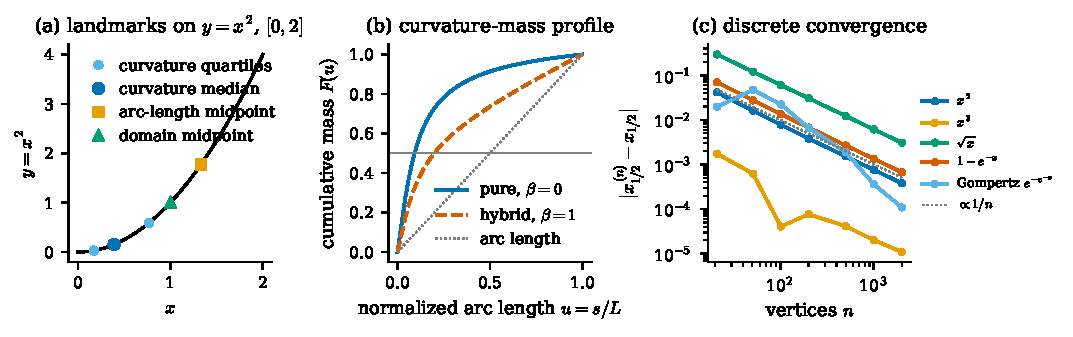
\includegraphics[width=\textwidth]{figures/fig1_concept.pdf}
\caption{(a) Landmarks on $y=x^2$, $x\in[0,2]$: the curvature median sits where the bending happens. (b) Pure and hybrid cumulative turning against normalized arc length. (c) Convergence of the discrete median to the exact values of \cref{tab:analytic}.}
\label{fig:concept}
\end{figure}

% =====================================================================
\section{Robustness of the landmarks}\label{sec:robust}

\subsection{Measurement noise}
We added Gaussian noise of standard deviation $\sigma$ (relative to the range of $y$) to $y=1-e^{-x}$ on $[0,4]$ with $n=201$ samples, \noiseTrials{} trials per level, and compare each estimator with its own noise-free value (\cref{tab:noise}). Without smoothing, the zigzags of the noise add turning everywhere and drag the median toward the middle of the domain; the error is about $\noiseRawWorst$ at every level, against a clean value of $\noiseCleanMedian$. After Savitzky--Golay smoothing \cite{savitzky1964} (window 51, cubic) the median is $\noiseKmaxRatioMin$ to $\noiseKmaxRatioMax$ times more stable than the location of maximum curvature, which is the expected advantage of an integral statistic over an argmax. In absolute terms, though, the smoothed median is only reliable at the lowest noise level here: by $\sigma=0.5\%$ its error approaches that of no smoothing at all. The hybrid median ($\beta=1$, clean value $\noiseCleanHybrid$) moves less, partly because it is pulled toward the arc-length midpoint and so has less room to move; it is a different landmark, not a better estimate of the same one. Curvature-based landmarks on sensor data require smoothing matched to the noise, and their precision should be reported, not assumed.

\begin{table}[t]
\centering\small
\caption{Mean absolute displacement (in $x$) of each landmark from its noise-free value, $y=1-e^{-x}$ on $[0,4]$, $n=201$.}
\label{tab:noise}
% AUTO-GENERATED -- do not edit by hand
\begin{tabular}{rcccc}
\toprule
$\sigma/\operatorname{range}(y)$ & median, raw & median, smoothed & hybrid median, smoothed & $\arg\max\kappa$, smoothed\\
\midrule
0.1\% & 1.285 & 0.155 & 0.107 & 0.603\\
0.5\% & 1.273 & 0.971 & 0.533 & 1.800\\
1.0\% & 1.226 & 1.116 & 0.643 & 2.107\\
2.0\% & 1.179 & 1.176 & 0.704 & 2.033\\
\bottomrule
\end{tabular}

\end{table}

\subsection{Window truncation}
For the logistic curve observed through asymmetric windows (\cref{tab:truncation}), the domain and arc-length midpoints follow the window ($\truncDomainMid$ and $\truncArcMid$ on $[-6,3]$) while the curvature median stays near the transition ($\truncMedian$). Its residual drift is governed by the boundary-angle mismatch $|\theta(b)-\theta(a)|$, in line with \cref{rem:sqrt}.

\begin{table}[t]
\centering\small
\caption{Landmarks of $y=1/(1+e^{-x})$ (inflection at $x=0$) under window truncation, $n=4001$.}
\label{tab:truncation}
\resizebox{\textwidth}{!}{% AUTO-GENERATED -- do not edit by hand
\begin{tabular}{crrrrr}
\toprule
window $[a,b]$ & $|\theta(b)-\theta(a)|$ (deg) & domain midpoint & arc-length midpoint & curvature median & hybrid median ($\beta=1$)\\
\midrule
$[-6.0,6.0]$ & 0.00 & $+0.000$ & $+0.000$ & $-0.000$ & $-0.000$\\
$[-6.0,3.0]$ & 2.45 & $-1.500$ & $-1.467$ & $-0.620$ & $-1.113$\\
$[-3.0,6.0]$ & 2.45 & $+1.500$ & $+1.467$ & $+0.620$ & $+1.113$\\
$[-2.0,4.0]$ & 4.98 & $+1.000$ & $+0.976$ & $+0.914$ & $+0.955$\\
$[-1.0,5.0]$ & 10.74 & $+2.000$ & $+1.970$ & $+1.466$ & $+1.792$\\
\bottomrule
\end{tabular}
}
\end{table}

\subsection{Several bends: the quantile gap}\label{sec:multi}
A single median is the wrong summary when the turning happens in separated places. For the double sigmoid $y=\sigma(x+d)+\sigma(x-d)$ on $[-12,12]$ the median stays at $0$, in the nearly straight stretch between the bends, for every $d$ (\cref{tab:multi}, \cref{fig:multi}). The quartiles track the two transitions ($\pm\quartileDSix$ at $d=6$), and the central gap $G_{0.05}$ grows from $\gapDOne$ at $d=1$ to $\gapDSix$ at $d=6$, a factor of $\gapRatio$: a flat stretch in $F$ at level $\tfrac12$ is the signature of a median sitting in a curvature desert.

\begin{table}[t]
\centering\small
\caption{Curvature quantiles ($x$-coordinates) and gaps (in normalized arc length) for the double sigmoid with separation $d$.}
\label{tab:multi}
% AUTO-GENERATED -- do not edit by hand
\begin{tabular}{rrrrrrcc}
\toprule
$d$ & $x(P_{0.25})$ & $x(P_{0.45})$ & $x(P_{0.50})$ & $x(P_{0.55})$ & $x(P_{0.75})$ & gap $P_{0.55}-P_{0.45}$ & $P_{0.75}-P_{0.25}$\\
\midrule
1 & $-2.40$ & $-1.05$ & $-0.00$ & $+1.05$ & $+2.40$ & 0.093 & 0.208\\
2 & $-3.42$ & $-1.03$ & $-0.00$ & $+1.03$ & $+3.42$ & 0.088 & 0.291\\
3 & $-3.92$ & $-1.13$ & $+0.00$ & $+1.13$ & $+3.92$ & 0.094 & 0.330\\
4 & $-4.56$ & $-1.62$ & $-0.00$ & $+1.62$ & $+4.56$ & 0.134 & 0.382\\
6 & $-6.14$ & $-3.18$ & $+0.00$ & $+3.18$ & $+6.14$ & 0.263 & 0.512\\
\bottomrule
\end{tabular}

\end{table}

\begin{figure}[t]
\centering
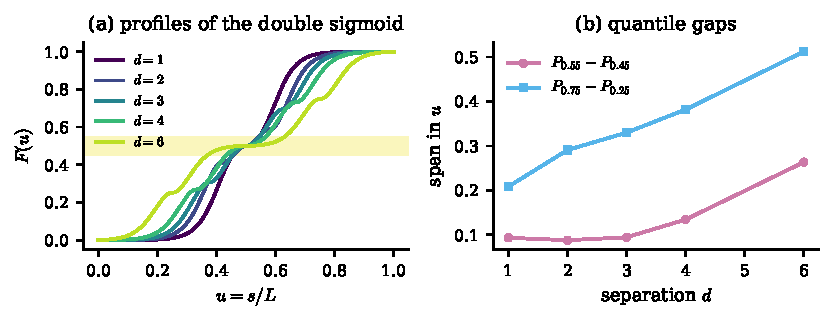
\includegraphics[width=0.78\textwidth]{figures/fig2_multi.pdf}
\caption{(a) Turning profiles of the double sigmoid develop a plateau at $F=\tfrac12$ as the bends separate. (b) The central quantile gap and the interquartile span.}
\label{fig:multi}
\end{figure}

% =====================================================================
\section{Comparing curves by their turning schedules}\label{sec:distance}

\Cref{tab:distance} shows $D$ (bold, above the diagonal) and $D_{1}$ (below) for six archetypes. Invariance holds to rounding: a copy rotated by $37^\circ$, scaled by $2.5$, and translated is at distance $\invarianceSimilarity$, and the same curve sampled with 157 instead of 601 points is at distance $\invarianceResample$, a discretization effect. The quantile and CDF forms of \cref{prop:w1} agree to within $\wOneIdentityMaxDiff$ over all pairs. Early and late bends are farthest apart ($D=\distEarlyLate$, $D_1=\distEarlyLateHybrid$).

Two cautions from \cref{fig:distance}. First, the U-bend and S-bend of \cref{sec:theory} have $D=\distUS$: identical unsigned schedules, different shapes. Second, on a nearly straight curve the pure distribution is dominated by tiny features. For $y=0.002x^2$ on $[0,1]$ (total turning $\dimpleTurningBase$ rad), adding a dimple of height $0.15\%$ moves the pure profile by $D=\dimplePure$, while the hybrid distance is $D_1=\dimpleHybrid$, \dimpleReduction\% smaller, because the arc-length component dominates when there is little turning.

\begin{table}[t]
\centering\small
\caption{Profile distances between archetypes: pure $D$ above the diagonal (bold), hybrid $D_1$ below.}
\label{tab:distance}
\resizebox{\textwidth}{!}{% AUTO-GENERATED -- do not edit by hand
\begin{tabular}{lccccccc}
\toprule
 & (1) & (2) & (3) & (4) & (5) & (6) & (7)\\
\midrule
(1) early bend & -- & \textbf{0.000} & \textbf{0.001} & \textbf{0.283} & \textbf{0.143} & \textbf{0.142} & \textbf{0.160}\\
(2) early, rotated+scaled & 0.000 & -- & \textbf{0.001} & \textbf{0.283} & \textbf{0.143} & \textbf{0.142} & \textbf{0.160}\\
(3) early, resampled & 0.001 & 0.001 & -- & \textbf{0.282} & \textbf{0.142} & \textbf{0.141} & \textbf{0.161}\\
(4) late bend & 0.161 & 0.161 & 0.160 & -- & \textbf{0.143} & \textbf{0.142} & \textbf{0.160}\\
(5) single sigmoid & 0.081 & 0.081 & 0.080 & 0.081 & -- & \textbf{0.121} & \textbf{0.152}\\
(6) double sigmoid & 0.081 & 0.081 & 0.081 & 0.081 & 0.069 & -- & \textbf{0.085}\\
(7) circular arc & 0.091 & 0.091 & 0.091 & 0.091 & 0.085 & 0.050 & --\\
\bottomrule
\end{tabular}
}
\end{table}

\begin{figure}[t]
\centering
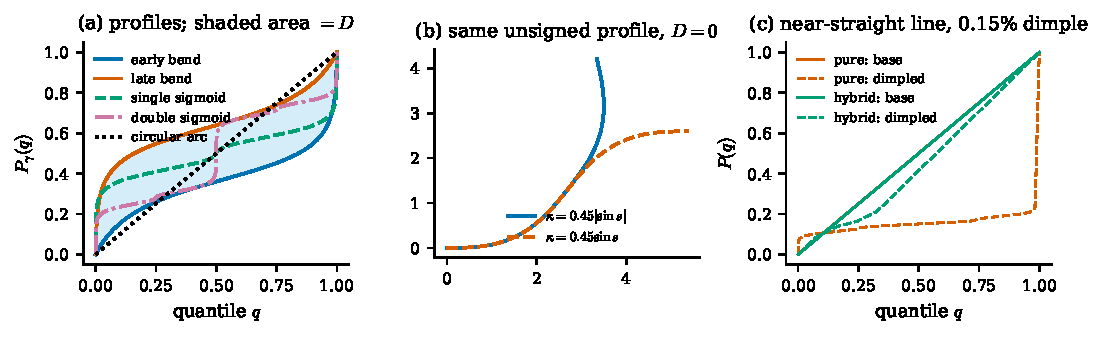
\includegraphics[width=\textwidth]{figures/fig3_distance.pdf}
\caption{(a) Quantile profiles of the archetypes; the shaded area is $D$ between the early and late bends. (b) Two curves with the same $|\kappa(s)|$ and therefore $D=0$. (c) A $0.15\%$ dimple on a nearly straight curve moves the pure profile a lot and the hybrid profile very little.}
\label{fig:distance}
\end{figure}

\subsection{Stroke classification}\label{sec:classify}
We generated \clsN{} open strokes, \clsPerClass{} in each of five classes (nodal-cubic ``alpha'', sine ``S'', circular ``C'', Archimedean spiral, and a straight-shaft ``J''), with random shape parameters, smooth low-frequency deformations, non-uniform sampling of 80 to 400 points, and a random rotation, scale ($0.5$ to $3$), and translation. \Cref{tab:classify} reports leave-one-out nearest-neighbour accuracy. Under mild perturbation every invariant descriptor, including $D$ and $D_1$, is perfect. Under strong perturbation the profile distances fall to $\clsHybridStrong\%$, while Procrustes alignment reaches $\clsProcrustesStrong\%$ and the signed turning function (with rotation removed) $\clsTurningStrong\%$. The unsigned profile throws away information the signed turning function keeps; its advantages are that it needs no alignment step and is a single 1-D integral. We do not claim it as a better classifier.

\begin{table}[t]
\centering\small
\caption{Leave-one-out 1-NN accuracy on \clsN{} synthetic strokes (5 classes).}
\label{tab:classify}
% AUTO-GENERATED -- do not edit by hand
\begin{tabular}{lcc}
\toprule
descriptor & mild & strong\\
\midrule
Euclidean, unaligned & 87.3\% & 83.3\%\\
Procrustes (rotation + scale) & 100.0\% & 98.0\%\\
turning function (Arkin et al.) & 100.0\% & 99.3\%\\
curvature profile $D$ (pure) & 100.0\% & 89.3\%\\
curvature profile $D_\beta$ ($\beta=1$) & 100.0\% & 89.3\%\\
\bottomrule
\end{tabular}

\end{table}

% =====================================================================
\section{Fixed-budget simplification by quantile resampling}\label{sec:resampling}

Given a polyline of $N$ vertices and a budget $K$, \emph{curvature-quantile (CQ) resampling} places output vertices at $P(q_k)$, $q_k=k/(K-1)$, for the measure $\mu_{p,\beta}$. With $p=\tfrac12$ and $\beta=0$ this equidistributes the classical asymptotically optimal density: a chord of length $\Delta s$ on an arc of curvature $\kappa$ deviates by about $\tfrac18|\kappa|\Delta s^2$, so equal deviation everywhere requires $\Delta s\propto|\kappa|^{-1/2}$ \cite{fejestoth1948,mcclure1975,glasauer1996}. The computation is one pass of edge vectors, angles, a prefix sum, and an interpolation, $O(N+K)$. Two variants matter in practice. \emph{Corner pinning} keeps every vertex whose turning angle exceeds $30^\circ$ and shares the remaining budget among the pieces between pinned vertices in proportion to their mass, which stops a uniform quantile grid from straddling and cutting a corner. \emph{Snapping} moves every output point to the nearest input vertex, turning resampling into decimation so that the comparison with vertex-subset methods is like for like.

\subsection{Protocol}
Nine curve families (\cref{tab:benchmark}: spiral, clothoid, corners with arcs, nearly straight line with two bumps, triple sigmoid, closed ellipse of eccentricity $0.987$, closed five-lobe Fourier star, closed self-intersecting Lissajous curve, and a mixed straight/looping/turning trajectory) are sampled with $N=\benchN$ vertices and normalized to unit size. Budgets are $K\in\{20,30,50,75,100\}$. The error is the largest distance from any input vertex to the simplified polyline (the directed Hausdorff distance, the usual simplification objective). Baselines are uniform arc-length resampling, VW by effective area, RDP driven to exactly $K$ vertices by always splitting the segment of largest deviation, and the exact optimum over vertex subsets with $K$ vertices, computed by dynamic programming in $O(N^3)$ time \cite{imai1986,perez1994,chin1996}. The optimum is a lower bound for any decimation method but not for resampling, which may place vertices between input vertices.

\subsection{Results}
\Cref{tab:benchmark} lists errors at $K=50$; the full grid is in the repository and summarized in \cref{fig:resampling}c. Over all \benchPairs{} family/budget pairs, CQ with $p=\tfrac12$ and corner pinning has a geometric-mean error ratio to RDP of $\benchGM$ (95\% bootstrap interval $[\benchCILo,\benchCIHi]$), wins $\benchWins$ pairs and loses $\benchLosses$ (exact two-sided Wilcoxon signed-rank $p=\benchWilcoxonP$). The losses occur in \benchLossFamilies. Six of the nine are at $K\le30$; the mixed trajectory, whose straight runs are interrupted by tight loops, also loses at $K=50$. Relative to the optimal vertex subset, CQ has a geometric-mean ratio of $\optRatioGM$ (range $\optRatioMin$ to $\optRatioMax$) against $\rdpOptRatioGM$ for RDP, and its snapped decimation variant keeps most of the gain over RDP (ratio $\snapGM$). Uniform arc-length resampling is $\uniformGM$ times worse than RDP and VW $\vwGM$ times worse.

The exponent matters. With $p=1$ (equal turning per segment, $\beta=1$) the ratio to RDP is $\cqOneGM$: equal turning per segment is the right schedule for locating bends but the wrong one for approximation. Corner pinning matters on polygonal content: on the corners-and-arcs family at $K=20$ unpinned CQ is $\cornerUnpinnedVsRDP\%$ worse than RDP because quantiles straddle the sawtooth corners, and pinning brings that to $\cornerPinnedVsRDP\%$; at $K=50$ and $K=75$ the pinned version matches or beats RDP on that family. Across all families, the geometric-mean ratio without pinning is $\cqUnpinnedGM$.

For the spiral with $K=50$, the setting of an earlier technical report, uniform, RDP, and CQ errors are $\spiralUniformFifty$, $\spiralRDPFifty$, and $\spiralCQHalfFifty$ (all $\times10^{-3}$), a $\spiralRedRDPFifty\%$ reduction from RDP.

\begin{table}[t]
\centering\small
\caption{Directed Hausdorff error ($\times10^{-3}$, unit-size curves) at $N=\benchN$, $K=50$. Best non-oracle method in bold; the optimal vertex subset (italic) is a lower bound for decimation methods only. CQ\,$1,\beta$: $p=1$, $\beta=1$. CQ\,$\frac12$: $p=\frac12$, $\beta=0$; ``pin'' adds corner pinning, ``snap'' snaps to input vertices.}
\label{tab:benchmark}
\resizebox{\textwidth}{!}{% AUTO-GENERATED -- do not edit by hand
\begin{tabular}{lrrrrrrrr}
\toprule
family & uniform & VW & RDP & CQ\,$1,\beta$ & CQ\,$\frac12$ & CQ\,$\frac12$ pin & CQ\,$\frac12$ snap & optimal\\
\midrule
F1 log spiral & 20.59 & 10.68 & 6.76 & 10.50 & \textbf{4.28} & \textbf{4.28} & 4.55 & \textit{4.14}\\
F2 clothoid & 4.35 & 4.18 & 3.45 & 5.20 & 2.12 & 2.12 & \textbf{2.09} & \textit{2.03}\\
F3 corners+arcs & 15.59 & 0.58 & 0.52 & 4.20 & 0.89 & \textbf{0.46} & 1.26 & \textit{0.30}\\
F4 line+bumps & 5.89 & 0.40 & 0.19 & 0.44 & \textbf{0.14} & \textbf{0.14} & 0.19 & \textit{0.12}\\
F5 triple sigmoid & 0.77 & 0.37 & 0.19 & 0.25 & \textbf{0.14} & \textbf{0.14} & 0.14 & \textit{0.10}\\
F6 ellipse (closed) & 11.33 & 1.32 & 0.59 & 1.41 & \textbf{0.31} & \textbf{0.31} & 0.34 & \textit{0.32}\\
F7 Fourier star (closed) & 20.81 & 9.80 & 6.54 & 10.14 & \textbf{4.18} & \textbf{4.18} & 4.27 & \textit{3.06}\\
F8 Lissajous (closed) & 14.19 & 10.44 & 5.43 & 7.52 & \textbf{2.94} & \textbf{2.94} & 3.03 & \textit{2.62}\\
F9 mixed trajectory & 9.02 & 2.26 & \textbf{2.06} & 5.61 & 3.49 & 3.49 & 3.64 & \textit{1.08}\\
\bottomrule
\end{tabular}
}
\end{table}

\begin{figure}[t]
\centering
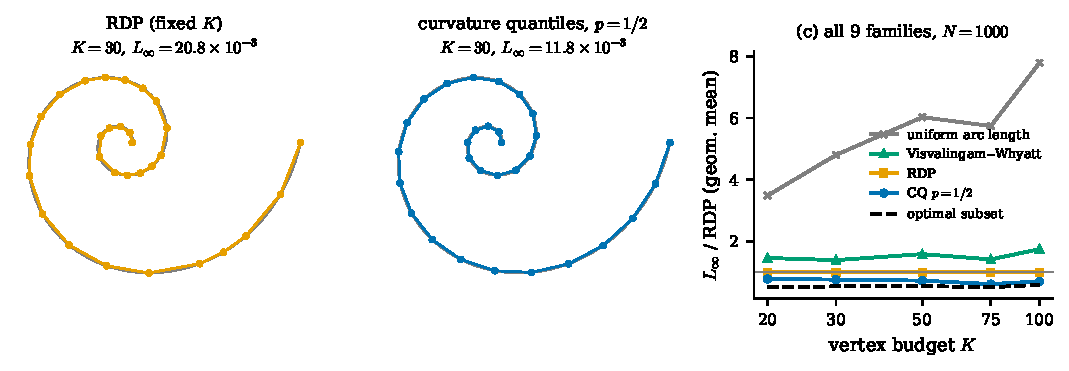
\includegraphics[width=\textwidth]{figures/fig4_resampling.pdf}
\caption{(a, b) Thirty vertices on the logarithmic spiral from RDP and from CQ resampling with $p=\tfrac12$. (c) Geometric mean over the nine families of the error ratio to RDP, by budget.}
\label{fig:resampling}
\end{figure}

\subsection{Noise}\label{sec:noise-resample}
\Cref{tab:noise-resample} repeats the comparison at $K=50$ on two families with Gaussian vertex noise of relative size $\eta$, measuring error against the clean curve (\noiseResampleTrials{} trials). On clean input CQ wins as above. With noise it does not: even after Savitzky--Golay smoothing (window 31, cubic), RDP on the smoothed input is better in every noisy case we ran. Residual noise inflates the turning mass along the gently curved parts, which pulls vertices away from where the true curvature is. Quantile resampling as presented here is a method for clean or well-filtered geometry (CAD paths, analytic or fitted curves), not for raw sensor tracks.

\begin{table}[t]
\centering\small
\caption{Error ($\times10^{-3}$) against the clean curve, $K=50$, $N=\benchN$, mean over trials. Smoothing is Savitzky--Golay, window 31, cubic.}
\label{tab:noise-resample}
% AUTO-GENERATED -- do not edit by hand
\begin{tabular}{llcccc}
\toprule
family & noise $\eta$ & RDP raw & CQ raw & RDP smoothed & CQ smoothed\\
\midrule
F1 log spiral & 0.0\% & 6.76 & 4.28 & 6.76 & 4.28\\
F1 log spiral & 0.2\% & 13.95 & 22.96 & 7.83 & 27.63\\
F1 log spiral & 0.5\% & 30.73 & 26.90 & 11.33 & 22.59\\
F1 log spiral & 1.0\% & 57.20 & 46.71 & 20.00 & 29.83\\
F4 line+bumps & 0.0\% & 0.19 & 0.14 & 0.19 & 0.14\\
F4 line+bumps & 0.2\% & 5.13 & 11.09 & 2.38 & 7.18\\
F4 line+bumps & 0.5\% & 10.81 & 11.36 & 4.65 & 8.91\\
F4 line+bumps & 1.0\% & 18.95 & 17.81 & 8.43 & 11.27\\
\bottomrule
\end{tabular}

\end{table}

\subsection{Cost}
CQ resampling is linear in $N$ with no recursion or heap. \Cref{tab:timing} gives single-threaded Python timings on the spiral with $K=N/50$. These are indicative only: CQ, uniform, and the inner loop of RDP are vectorized NumPy, VW is a pure-Python heap, and a compiled implementation would change all four columns.

\begin{table}[t]
\centering\small
\caption{Median wall-clock time (ms) of the reference implementations.}
\label{tab:timing}
% AUTO-GENERATED -- do not edit by hand
\begin{tabular}{rrrrrr}
\toprule
$N$ & $K$ & uniform & CQ & RDP & VW\\
\midrule
1{,}000 & 20 & 0.03 & 0.16 & 0.29 & 5.73\\
10{,}000 & 200 & 0.11 & 0.58 & 3.11 & 63.72\\
100{,}000 & 2{,}000 & 1.41 & 7.72 & 31.74 & 1033.74\\
\bottomrule
\end{tabular}

\end{table}

% =====================================================================
\section{Discussion}\label{sec:discussion}

Treating $|\kappa|\dd s$ as a distribution gives a small, coherent vocabulary for where curves turn: medians with closed forms on convex arcs, quantile gaps that flag separated bends, and a transport distance that is invariant by construction. The theory is elementary and several pieces overlap with earlier work, which we have tried to credit precisely: the cumulative distribution is Tumpach's curvature-proportional parameterization \cite{tumpach2023canonical}, the distance is a turning-function distance on convex arcs \cite{arkin1991metric}, and the $|\kappa|^{1/2}$ density is classical \cite{mcclure1975}. Two findings were not in our starting notes and may be the most useful to others: the square-root sensitivity of the median at an inflection (\cref{rem:sqrt}), and the measured gap between equal-quantile resampling and the true optimum over vertex subsets.

The limitations are as important as the results. The unsigned measure discards chirality, so $D$ cannot separate an S from a U. The profile distance on closed curves depends on the start point unless a circular transport distance is used \cite{delon2009circle}. Every curvature statistic here is sensitive to noise and needs smoothing whose scale must be chosen. The simplification benchmark is synthetic; real-data evaluation on GPS tracks, coastlines, or CNC toolpaths, comparison with reduced-search dynamic programming \cite{kolesnikov2003}, and a compiled implementation are natural next steps, as is a comparison with elastic shape analysis \cite{srivastava2011elastic} and curvature scale space \cite{mokhtarian1992} for shape retrieval.

\section*{Reproducibility}
The Python package \texttt{curvquant}, unit tests, and the script \texttt{experiments/run\_all.py} that regenerates every number, table, and figure in this note are available at \repo. Numbers in the text are inserted automatically from the script's output.

\section*{Acknowledgments}
The author used AI assistants for exploratory computation, literature search, and drafting; every number in this version is recomputed by the released code.

\bibliographystyle{plainnat}
\bibliography{refs}

\end{document}
